\chapter{Evaluation und Optimierung bestehender Locks}
\label{ch:benchmarks}

Das wohl wichtigste Kriterium für den Vergleich von Locks
ist die Geschwindigkeit der Implementierung.
Ein schnellerer Lock ist natürlich besser,
aber die Geschwindigkeit hängt nicht nur vom Algorithmus und der Hardware ab,
sondern auch davon,
in welchem Kontext der Lock aufgerufen wird.
Es kann zum Beispiel einen Unterschied machen,
wie viele Prozesse gleichzeitig versuchen,
den Lock zu akquirieren (\gls{Konkurrenz})
oder ob der Prozess,
der den Lock als Letztes hatte,
auf demselben Rechenknoten lief.
Es gibt daher zahlreiche verschiedene Szenarien in der Literatur,
in denen Benchmarks durchgeführt werden.
Hierbei kann man zwischen einfachen synthetischen Benchmarks
und der Integration in eine bestehende Anwendung unterscheiden.

Eine Integration in eine bestehende Anwendung hat den Vorteil,
dass das Szenario realistischer ist
und die Ergebnisse somit besser den realen Nutzen zeigen.
Leider steht im Rahmen dieser Arbeit keine Anwendung zur Verfügung,
in die die Locks integriert werden könnten.

Synthetische Benchmarks sind sehr fein granular
und können daher gezielt bestimmte Aspekte einer Implementierung analysieren.
Beispielsweise kann man nur mit einem synthetischen Benchmark messen,
wie lange es dauert,
einen freien Lock zu akquirieren.
Außerdem laufen sie schneller,
da nur genau das ausgeführt wird,
was für den Benchmark notwendig ist.
Eine Sammlung solcher Benchmarks
in einer Programmbibliothek
wird im Folgenden als Benchmarksuite bezeichnet.

In der Literatur \cite{RH-Lock} \cite{HCLH-Lock} \cite{FC-MCS-Lock} \cite{RCL} \cite{SANL} \cite{RMA-RW}
wird für synthetische Benchmarks meist eine festgelegte Anzahl an Iterationen definiert.
In einer Schleife akquiriert ein Prozess den Lock
und führt je nach Benchmark noch andere Operationen aus.
Dabei wird die Zeit gemessen,
bis alle Prozesse fertig sind.
Im Gegensatz dazu wird in dieser Arbeit (analog zu \cite{Cohort-Lock}, \cite{CNA-Lock} und \cite{Shfl-Lock}) eine Zeit vorgegeben
und nach jeder Iteration geprüft,
ob diese Zeit schon abgelaufen ist.
Das hat den Nachteil,
dass jede Iteration zusätzlichen Overhead durch eine Abfrage der Systemzeit erfährt.
Dieser Overhead hat allerdings nur eine Größenordnung von einigen Nanosekunden (ns),
während die Dauer von \gls{rma}-Zugriffen auf entfernten Speicher in der Größenordnung von Mikrosekunden (\textmu{s}) liegt.
Der Vorteil dieser Variante ist,
dass dadurch eine empirische Analyse der Fairness (siehe \autoref{sec:fairness_empirisch}) möglich wird.
In dieser Arbeit wird für solche Benchmarks eine Laufzeit von einer Sekunde pro Lock und Prozessanzahl verwendet,
wobei die ersten 10~\% der Zeit nicht in die Messung eingehen,
sondern zum Aufwärmen dienen.

Jeder Benchmark wird acht Mal ausgeführt.
Gezeigt wird immer der Median dieser Ausführungen mit 95~\% Konfidenzintervall.
In dieser Arbeit wird der Median verwendet,
da dieser im Gegensatz zum arithmetischen Mittel nicht von Ausreißern beeinflusst wird.
Solche Ausreißer können auf einem verteilten System mit vielen Nutzern leicht auftreten
und würden sonst das Messergebnis verfälschen.
Durch die Angabe der Konfidenzintervalle ist außerdem ersichtlich,
wie groß die Abweichung des Medians zwischen den einzelnen Läufen war.
Mit dieser Information konnten bei der Erstellung dieser Arbeit einige Benchmarkergebnisse identifiziert werden,
die wegen hoher Auslastung des Rechenzentrums enorme Schwankungen aufwiesen.
Diese Benchmarks wurden dann zu einem späteren Zeitpunkt wiederholt.

Alle Benchmarks wurden auf dem CoolMUC-2 Linux Cluster des \gls{lrz} ausgeführt%
\footnote{\url{https://doku.lrz.de/display/PUBLIC/CoolMUC-2}}.
Dieses Cluster nutzt Intels Haswell Prozessoren mit einer Taktfrequenz von 2,6 GHz
und hat 28 Kerne pro Rechen-knoten mit je 2 Hyperthreads.
Die Knoten sind mit FDR14 Infiniband verbunden.
Die Verbindung hat eine Latenz von 2,3~\textmu{s}
und eine Bandbreite von 13,64 GB/s pro Knoten.
Als \gls{mpi}-Implementierung wurde Intel-MPI%
\footnote{Intel(R) MPI Library for Linux* OS, Version 2019 Update 10 Build 20210120 (id: d7908565b)}
verwendet und die Benchmarks wurden mit ICPC%
\footnote{icpc (ICC) 19.1.2.254 20200623}
kompiliert.

Um die Effekte von Hyperthreading zu vermeiden,
wurden in den Benchmarks maximal 28 Prozesse auf einem exklusiv reservierten Rechenknoten ausgeführt.
Jeder Knoten erhielt dabei stets die gleiche Anzahl an Prozessen.

\section{Vergleichskriterien}
\label{sec:kriterien}

Um die verschiedenen Algorithmen und Optimierungen objektiv miteinander vergleichen zu können,
müssen zunächst die Vergleichskriterien definiert werden.
Der Fokus liegt in dieser Arbeit auf dem Vergleich der Geschwindigkeit,
aber es wird auch die Fairness empirisch untersucht.
% Speicherverbrauch wird nur kurz in \autoref{sec:speicherverbrauch} behandelt.

\subsection{Geschwindigkeit}
\label{sec:geschwindigkeit}

Die Geschwindigkeit der Implementierungen ist das wichtigste Vergleichskriterium.
Im Rahmen dieser Arbeit wird manchmal die durchschnittliche Dauer einer Iteration betrachtet
und manchmal invers dazu der Durchsatz,
also wie viele kritische Abschnitte pro Sekunde ausgeführt werden.
Je nach Szenario ist die eine oder die andere Betrachtungsweise geeigneter,
um die Unterschiede zwischen zwei Implementierungen herauszustellen.
Beide Darstellungen zeigen aber dieselben Daten
und können leicht durch Berechnung von $y \rightarrow \frac{1}{y}$ ineinander umgewandelt werden.

\subsection{Konkurrenz}
\label{sec:contention}

Die \glsfirst{Konkurrenz} ist kein direktes Vergleichskriterium,
hat aber einen großen Einfluss auf das Verhalten eines Locks
und hilft daher bei der Interpretation der Geschwindigkeit.
Bei großer \gls{Konkurrenz} muss ein Prozess z.~B. länger warten,
bis der Lock freigegeben wird.
Außerdem muss ein Prozess bei vielen Algorithmen andere Codepfade durchlaufen,
wenn eine geringe \gls{Konkurrenz} vorliegt.
Z.~B. muss bei der Freigabe eines MCS-Locks
der \texttt{tail}-Zeiger nur dann zurückgesetzt werden,
wenn noch kein Nachfolger wartet (vgl. \autoref{fig:mcs_release}).

Die verschiedenen Benchmarks setzen die Locks verschiedenen \gls{Konkurrenz}situationen aus.
Um die tatsächliche \gls{Konkurrenz} quantifizieren zu können,
wird sie definiert als:
der Anteil der Akquisitionen,
bei denen ein Prozess den Lock nicht direkt akquirieren konnte,
sondern auf einen Vorgänger warten musste.
Die \gls{Konkurrenz} geht also von 0~\% bis 100~\%
und es wird nicht unterscheiden,
wie viele Prozesse bei einer \gls{Konkurrenz} von 100~\% versuchen,
den Lock zu akquirieren.

Diese Messung muss in die Lock-Implementierung eingebaut werden,
da sonst nicht ersichtlich ist,
ob auf einen Vorgänger gewartet wurde.
Daher ist leider keine Messung der \gls{Konkurrenz} bei Locks aus Bibliotheken wie z.~B. DASH möglich.

\subsection{Fairness}
\label{sec:fairness_empirisch}

Neben der Geschwindigkeit ist auch die Fairness ein wichtiges Vergleichskriterium.
Fairness wird häufig nur auf theoretischer Ebene betrachtet (vgl. \autoref{sec:fairness_theoretisch}).
In dieser Arbeit geht es aber nicht um die theoretische Fairness der Lock-Algorithmen,
sondern um die praktische Fairness der Lock-Implementierungen.

Um diese zu messen wird wie in \cite{Cohort-Lock} gezählt,
wie viele Iterationen des Benchmarks jeder Prozess in der gegebenen Zeit ausführt.
Damit erhält man den Programmfortschritt,
also wie weit jeder einzelne Prozess ein Programm ausführen würde.
Um nun die Fairness zu bewerten wird der empirische Variationskoeffizient (engl. \gls{cv}) der einzelnen Programmfortschritte bestimmt.
Dieser berechnet sich aus der Standardabweichung $\sigma$ und dem Durchschnitt $\mu$ mit $\frac{\sigma}{\mu}$.
Da es sich um eine Stichprobe handelt wird Bessels Korrektur \cite{bessels_correction} bei der Berechnung der Varianz (und damit der Standardabweichung) verwendet.
Ein geringerer Variationskoeffizient ist somit besser,
da er eine geringere Abweichung des Programmfortschritts
und damit einen faireren Lock bedeutet.

Im Gegensatz zur Standardabweichung hat der Variationskoeffizient keine Einheit
und ist somit unabhängig von der gemessenen Größe.
Er eignet sich daher auch gut,
um die Fairness von zwei Locks zu vergleichen,
die eine sehr unterschiedliche Performance
und damit auch sehr unterschiedliche Standardabweichungen des Programmfortschritts haben.

% Wie auch bei den Messungen der Geschwindigkeit und der \gls{Konkurrenz},
% wird für den Variationskoeffizienten der Median der acht Wiederholungen des Benchmarks mit 95~\% Konfidenzintervall angegeben.

\section{Evaluation bestehender Locks}

Zunächst werden die aktuell auf verteiltem Speicher zur Verfügung stehenden Locks evaluiert,
da diese die Basis darstellen,
gegen die alle portierten Locks verglichen werden müssen:\begin{enumerate}
    \item \enquote{MPI}: Der Lock der \gls{mpi}-Implementierung: \texttt{MPI\_Win\_lock} mit einem \texttt{MPI\_Get} und \texttt{MPI\_Win\_flush} (siehe \autoref{sec:mpi_locks}).
    \item \enquote{DASH}: \texttt{dash::Mutex} aus \cite{DART-MPI}.
          Hierbei handelt es sich um eine Variante eines MCS-Locks mit Punkt-zu-Punkt-Kommunikation für die Übergabe des Locks an den Nachfolger (siehe \autoref{sec:p2p_lock_passing}).
    \item \enquote{D-MCS}: Die Implementierung eines MCS-Locks aus \cite{RMA-RW},
          erweitert um\\\texttt{MPI\_Iprobe} (siehe \autoref{sec:mpi_fortschritt}).
    \item \enquote{RMA-MCS}: Die Implementierung eines HMCS-Locks \cite{HMCS-Lock} aus \cite{RMA-RW} erweitert um \texttt{MPI\_Iprobe} (siehe \autoref{sec:mpi_fortschritt}).
\end{enumerate}
Da es bisher kaum Forschung zu Locks in verteiltem Speicher gibt,
gibt es hierfür auch keine umfangreiche Benchmarksuite.
Daher wurden Szenarien aus \cite{RMA-RW} und einigen Arbeiten über \gls{numa}-Locks
auf verteilten Speicher übertragen und angepasst.
Der Quelltext der Benchmarks und Locks aus dieser Arbeit ist auf GitHub veröffentlicht:\\
\url{https://github.com/Adrodoc/distributed-locks}

\subsection{Performance freier Locks (UPB)}
\label{sec:upb}

Für Anwendungen,
in denen nur selten mehrere Prozesse gleichzeitig einen kritischen Abschnitt betreten möchten,
ist es besonders wichtig,
dass ein freier Lock sehr schnell akquiriert und wieder freigegeben werden kann.
Dies wird mit dem \gls{upb} aus \cite{RH-Lock} gemessen.

Die meisten Locks haben einen Hauptprozess,
auf dessen Speicher beim Akquirieren immer zugegriffen wird.
Das ist z.~B. beim MCS-Lock der Prozess,
in dessen Speicher der Zeiger liegt,
der auf das Ende der Warteschlange zeigt.
Daher macht es einen Unterschied,
ob der freie Lock von dem Hauptprozess akquiriert wird,
von einem anderen Prozess auf demselben Knoten (dem Hauptknoten)
oder von einem Prozess auf einem anderen Knoten.
Im letzten Fall ist für das Akquirieren sogar ein Zugriff auf entfernten Speicher nötig.
Beim RH-Lock (siehe \autoref{sec:rh-lock}) macht es außerdem einen Unterschied,
welcher Prozess zuletzt den Lock akquiriert hatte.
Damit ergeben sich insgesamt die neun Szenarien in \autoref{tab:upb_szenarien}.

\begin{table}[h]
    \centering
    \begin{tabular}{|c|c|c|c|}
        \hline
        \diagbox{Vorgänger}{Hauptprozess} & Selber Prozess & Selber Knoten & Anderer Knoten \\
        \hline
        Selber Prozess                    & 1a             & 1b            & 1c             \\
        \hline
        Selber Knoten                     & 2a             & 2b            & 2c             \\
        \hline
        Anderer Knoten                    & 3a             & 3b            & 3c             \\
        \hline
    \end{tabular}
    \caption{UPB-Szenarien}
    \label{tab:upb_szenarien}
\end{table}

Anders als die anderen Benchmarks in dieser Arbeit nutzt der \gls{upb} nicht einen Lock,
der in einer Schleife immer wieder verwendet wird,
sondern viele Locks,
die für eine Messung jeweils nur einmal verwendet werden.
So wird sichergestellt,
dass die Locks frei sind
und je nach Szenario den entsprechenden Vorgänger hatten.
In dieser Arbeit werden hierfür 1000 Locks verwendet.
Um alle Szenarien durchführen zu können,
werden 4 Prozesse benötigt,
von denen jeweils 2 auf demselben Knoten laufen müssen.
Da die Locks im \gls{upb} immer frei sind,
ist die \gls{Konkurrenz} immer 0
und es kann keine Fairness gemessen werden.
Im \gls{upb} wird daher nur die Geschwindigkeit untersucht.

\begin{figure}[h]
    \centering
    \begin{tabular}{c}\begin{lstlisting}
        // Aufwärmen
        acquire_and_release_all_locks(locks);
        MPI_Barrier(comm);

        // Mache Prozess 4 zum Vorgänger
        if (rank == 4)
          acquire_and_release_all_locks(locks);
        MPI_Barrier(comm);

        // Szenario 3a:
        if (rank == 0)
          dauer_3a = acquire_and_release_all_locks(locks);
        MPI_Barrier(comm);

        // Szenario 1a: ...
    \end{lstlisting}\end{tabular}
    \caption{Anfang vom Quelltext des UPBs (\upburl)}
    \label{fig:upb_code}
\end{figure}

\autoref{fig:upb_code} zeigt den Anfang vom Quelltext des \gls{upb}s.
In diesem Beispiel hat der Hauptprozess aller Locks $rank = 0$
und läuft zusammen mit dem Prozess mit $rank = 1$ auf dem Hauptknoten.
Zum Aufwärmen werden zunächst alle Locks von allen Prozessen einmal akquiriert und wieder freigegeben.
Anschließend akquiriert der Prozess mit $rank = 4$ alle Locks,
damit alle Locks einen definierten Vorgänger haben.
Schließlich werden die Szenarien in folgender Reihenfolge ausgeführt: 3a, 1a, 2b, 1b, 2a, 3c, 1c, 2c, 3b.
Die Reihenfolge ist so gewählt,
dass in jedem Szenario die Locks den korrekten Vorgänger hatten.

\begin{benchmark}[h]
    \begin{subfigure}{.5\textwidth}
        \includegraphics[width=\textwidth]{benchmarks/intelmpi/baseline/UPB-lock_count=1000-latency}
        \caption{Iterationsdauer in \textmu{s}}
        \label{ben:baseline_upb_latency}
    \end{subfigure}
    \begin{subfigure}{.5\textwidth}
        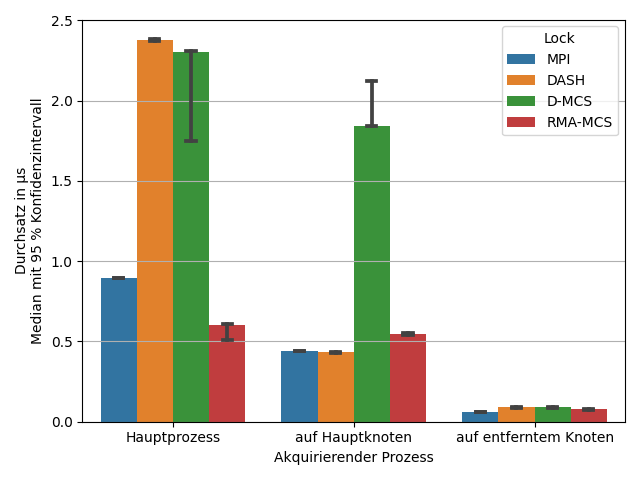
\includegraphics[width=\textwidth]{benchmarks/intelmpi/baseline/UPB-lock_count=1000-throughput}
        \caption{Durchsatz in Mio/s}
        \label{ben:baseline_upb_throughput}
    \end{subfigure}
    \caption{UPB der Basislocks}
    \label{ben:baseline_upb}
\end{benchmark}

\autoref{ben:baseline_upb_latency} zeigt,
wie lange es durchschnittlich dauert,
einen freien Lock zu akquirieren.
\autoref{ben:baseline_upb_throughput} hingegen zeigt umgerechnet,
wie viele Millionen freie Locks pro Sekunde akquiriert werden können.
Da es für diese Locks keinen Unterschied macht,
welcher Prozess der Vorgänger war,
sind in den beiden Abbildungen die Messungen unabhängig vom Vorgänger zusammengefasst.
Die Konfidenzintervalle beziehen sich hier somit auf 24 Messungen,
statt wie sonst auf 8.

In den Abbildungen sieht man deutlich den Einfluss von entfernten Speicherzugriffen auf die Performance.
Wenn der Hauptprozess des Locks auf einem anderen Knoten läuft
als der Prozess,
der den Lock akquiriert und freigibt,
sind alle Locks deutlich langsamer.
Beim Intel-MPI-Lock und \texttt{dash::Mutex} macht es darüber hinaus einen großen Unterschied,
ob der Prozess selbst der Hauptprozess
oder ein anderer Prozess auf dem Hauptknoten ist.
Der Grund hierfür ist leider nicht bekannt.
Zumindest bei \texttt{dash::Mutex} liegt es jedenfalls nicht an dem verwendeten Algorithmus,
denn sowohl \texttt{dash::Mutex}
als auch D-MCS müssen in diesem Benchmark nur zwei \gls{mpi}-Operationen ausführen:
ein \texttt{MPI\_Fetch\_and\_op} zum Akquirieren
und ein \texttt{MPI\_Compare\_and\_swap} zum Freigeben (jeweils mit \texttt{MPI\_Win\_flush}).
In \autoref{sec:optimierung_bestehender_locks} wird gezeigt,
dass eine Reimplementierung des Algorithmus aus \texttt{dash::Mutex} dieses Verhalten nicht aufweist.

Außerdem zeigt der \gls{upb},
dass ein freier RMA-MCS-Lock immer etwas langsamer ist
als ein freier D-MCS-Lock.
% Das ist auch zu erwarten.
Da RMA-MCS eine hierarchische Version des D-MCS mit zwei Hierarchieebenen ist,
muss bei einem freien Lock sowohl der lokale Lock
als auch der globale Lock akquiriert werden,
während D-MCS nur aus einem globalen Lock besteht.
\autoref{ben:baseline_upb_latency} zeigt allerdings,
dass der Overhead
von RMA-MCS gegenüber D-MCS
nur bei etwa 1,5~\textmu{s} liegt und zwar unabhängig davon,
auf welchem Knoten der Prozess läuft.

\clearpage

\subsection{Leerer kritischer Abschnitt (ECSB)}
\label{sec:ecsb}

Der Benchmark mit leerem kritischen Abschnitt (engl. \gls{ecsb}) ist
% in der Literatur
sehr verbreitet \cite{RH-Lock} \cite{HCLH-Lock} \cite{FC-MCS-Lock} \cite{HMCS-Lock},
vermutlich, weil er sehr einfach ist.
In einer Schleife akquiriert jeder Prozess den Lock
und gibt ihn direkt wieder frei.
Das ist zwar nicht sehr realistisch,
dafür beeinflusst aber nur der Lock selbst die Messung.
% denn es gibt keinen Overhead durch andere Operationen.

\begin{benchmark}[h]
    \begin{subfigure}{.5\textwidth}
        \includegraphics[width=\textwidth]{benchmarks/intelmpi/baseline/ECSB-latency}
        \caption{Iterationsdauer in \textmu{s}}
        \label{ben:baseline_ecsb_latency}
    \end{subfigure}
    \begin{subfigure}{.5\textwidth}
        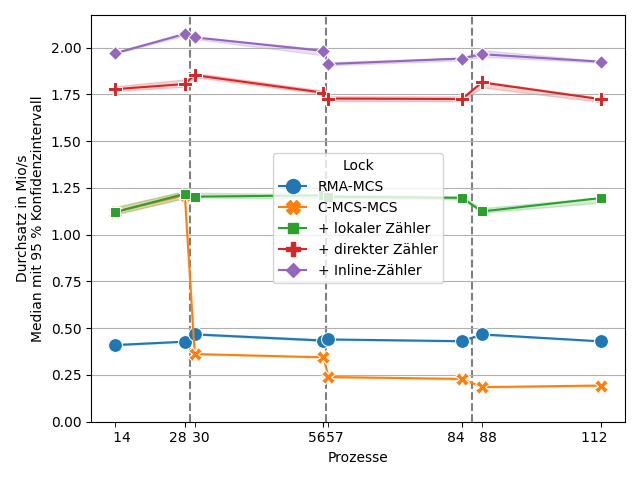
\includegraphics[width=\textwidth]{benchmarks/intelmpi/baseline/ECSB-throughput}
        \caption{Durchsatz in Mio/s}
        \label{ben:baseline_ecsb_throughput}
    \end{subfigure}
    \caption{ECSB der Basislocks (\ecsburl)}
    \label{ben:baseline_ecsb}
\end{benchmark}

\autoref{ben:baseline_ecsb} zeigt die Performance der Locks im \gls{ecsb}.
Man sieht,
dass in diesem Benchmark der Lock aus Intel-MPI bei Weitem am schnellsten ist,
solange nur ein Rechenknoten beteiligt ist.
Hier besteht offenbar großes Optimierungspotenzial bei den anderen Locks.
Jedes Mal,
wenn ein weiterer Rechenknoten hinzukommt
(bei 30, 57 und 88 Prozessen)
nimmt die Geschwindigkeit des MPI-Locks jedoch stark ab.
\texttt{dash::Mutex} zeigt ein sehr ähnliches Verhalten.
Hier ist allerdings auffällig,
dass dieser Lock hohe Schwankungen aufweist.
D-MCS und RMA-MCS sind bei mehreren Knoten deutlich schneller,
da sie direkte Speicherzugriffe
statt \gls{rma}-Operationen in den Warteschleifen verwenden (siehe \autoref{sec:mpi_fortschritt}).

Es wird auch deutlich,
dass Zugriffe auf entfernten Speicher vermieden werden sollten.
D-MCS unterscheidet nicht zwischen Prozessen auf demselben und anderen Knoten.
Die Performance nimmt daher bei 30 Prozessen deutlich ab,
da dann mehr als ein Rechenknoten beteiligt ist,
bleibt aber bei weiteren Knoten relativ konstant.
RMA-MCS verhält sich als einzige Implementierung stabil,
unabhängig von der Anzahl der Prozesse und Rechenknoten.

Da beim \gls{ecsb} außerhalb des kritischen Abschnitts nichts gemacht wird,
versuchen ständig Prozesse den kritischen Abschnitt zu betreten
und der Lock ist nie frei.
Die \gls{Konkurrenz} (nicht gezeigt) ist daher bei allen Locks unabhängig von der Anzahl an Prozessen bei 100~\%.

\begin{benchmark}[h]
    \centering
    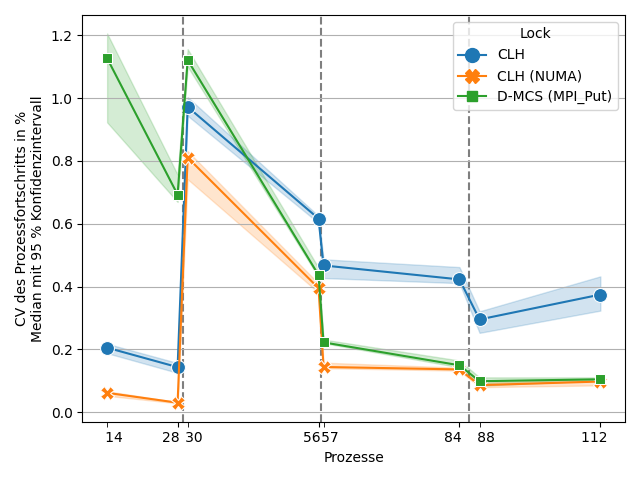
\includegraphics[width=.5\textwidth]{benchmarks/intelmpi/baseline/ECSB-fairness}
    \caption{Fairness der Basislocks im ECSB: CV des Fortschritts in \%}
    \label{ben:baseline_ecsb_fairness}
\end{benchmark}

\autoref{ben:baseline_ecsb_fairness} zeigt die Fairness der Locks im \gls{ecsb}.
Obwohl \texttt{dash::Mutex} und D-MCS beides Varianten des MCS-Locks sind
und theoretisch \gls{fifo} garantieren,
weist D-MCS eine etwas schlechtere Fairness auf,
die bei mehr und mehr Prozessen aber zu \texttt{dash::Mutex} aufholt.
RMA-MCS hat theoretisch eine beschränkte Unfairness von 50,
d.~h. es können maximal 50 andere Prozesse den ersten Prozess in der Warteschlange überholen.
Diese schlechtere theoretische Fairness könnte auch der Grund für die etwas schlechtere praktische Fairness sein.
Der Intel-MPI-Lock ist bei mehreren Knoten mit Abstand am unfairsten,
alle Locks sind mit einem Variationskoeffizienten von deutlich unter 5 \% allerdings ziemlich fair.

\subsection{Änderung des kritischen Arbeitsanteils (CCWB)}
\label{sec:ccwb}

Einen deutlich realistischeren Ansatz hat der \gls{ccwb}.
Auch dieser wird in verschiedenen Varianten häufig in der Literatur verwendet
\cite{RH-Lock} \cite{HCLH-Lock} \cite{FC-MCS-Lock} \cite{Cohort-Lock} \cite{RCL} \cite{HMCS-Lock} \cite{SANL}.
Die Idee bei diesem Benchmark ist es,
die \gls{Konkurrenz} zwischen den Prozessen zu erhöhen,
indem ein immer größerer Anteil der Arbeit im kritischen Abschnitt ausgeführt wird,
bis diese den Hauptteil der Rechenzeit beansprucht.
Zunächst ist der kritische Abschnitt leer.
Anders als beim \gls{ecsb} führen Prozesse aber vor dem Akquirieren des Locks einige Speicherzugriffe aus.
Diese Zugriffe repräsentieren den parallelisierbaren Anteil eines Programms
und werden im Folgenden als unkritische Arbeit $u$ bezeichnet.
Dann werden mehr und mehr Operationen im kritischen Abschnitt ausgeführt,
wodurch ein immer größerer Anteil des Programms serialisiert werden muss
und immer mehr Prozesse gleichzeitig den kritischen Abschnitt ausführen wollen.
Diese Operationen werden
% im Folgenden
als kritische Arbeit $k$ bezeichnet.
\autoref{fig:ccwb_code} zeigt den Quelltext einer \gls{ccwb}-Iteration.

\begin{figure}[h]
    \centering
    \begin{tabular}{c}\begin{lstlisting}
void ccwb(Lock &lock) {
  lock.acquire();
  for (int i = 0; i < k; i++)
    increment_non_atomically(sizeof(int) * i);
  lock.release();
  int u = distribution(generator);
  for (int i = 0; i < u; i++)
    increment_non_atomically(sizeof(int) * (k + i));
}

void increment_non_atomically(MPI_Aint disp) {
  // Der \enquote{rank} eines Prozesses, der wahrscheinlich auf einem anderen Knoten läuft.
  int remote_rank = (my_rank + p / 2) % p;
  int value;
  MPI_Get(&value, 1, MPI_INT, remote_rank, disp, 1, MPI_INT, win);
  MPI_Win_flush(remote_rank, win);
  value += 1;
  MPI_Put(&value, 1, MPI_INT, remote_rank, disp, 1, MPI_INT, win);
  MPI_Win_flush(remote_rank, win);
}
    \end{lstlisting}\end{tabular}
    \caption{Quelltext einer CCWB Iteration (\ccwburl)}
    \label{fig:ccwb_code}
\end{figure}

Ein spannender Punkt ist erreicht,
wenn kritische und unkritische Arbeit gleichermaßen an der Laufzeit beteiligt sind.
Das ist der Fall,
wenn die unkritische Arbeit $p - 1$ Mal so groß ist
wie die kritische Arbeit,
wobei $p$ die Anzahl der Prozesse ist.
Damit stellt die kritische Arbeit einen Anteil von $\frac{1}{p}$ der gesamten Arbeit eines Prozesses dar.
Dies ist der letzte Punkt,
an dem das Programm theoretisch perfekt parallelisierbar ist und wird im Folgenden als Equilibrium bezeichnet.

Man kann sich vorstellen,
dass im Optimalfall immer ein Prozess den kritischen Abschnitt ausführt,
während die anderen $p - 1$ Prozesse unkritische Arbeit ausführen.
In der Realität ist bereits etwas früher keine perfekte Parallelisierung mehr möglich,
da die Prozesse nicht immer zum perfekten Zeitpunkt den kritischen Abschnitt betreten möchten
und das Akquirieren und Freigeben des Locks zusätzlich Zeit benötigt.

Echte Anwendungen brauchen nicht zwischen jedem kritischen Abschnitt die gleiche Anzahl an Operationen.
Um das zu simulieren wird die tatsächliche Menge der unkritischen Arbeit zufällig bestimmt.
Ausgehend von einer minimalen Anzahl an Operationen $a$ bestimmt jeder Prozess in jeder Iteration
seine tatsächliche Arbeit $\tilde{a}$ indem er über eine Gleichverteilung eine Zufallszahl aus dem geschlossenen Intervall $[a; 2a]$ bestimmt.
Dies geschieht vor dem kritischen Abschnitt und nutzt \texttt{std::mt19937}%
\footnote{\url{https://en.cppreference.com/w/cpp/numeric/random/mersenne_twister_engine}}
und \texttt{std::uniform\_int\_distribution}%
\footnote{\url{https://en.cppreference.com/w/cpp/numeric/random/uniform_int_distribution}}
aus C++.
Die unkritische Arbeit $u$ bestimmt sich dann mit $u = \tilde{a} - k$.

Nun soll $a$ so gewählt werden,
dass das Equilibrium $e$ im Durchschnitt bei einer kritischen Arbeit von $k = 3$ erreicht ist.
So kann bei $k \in [0; 2]$ beobachtet werden,
wie der Lock sich verhält,
wenn die unkritische Arbeit dominiert
und bei $k \in [4; 5]$,
wie er sich verhält,
wenn die kritische Arbeit dominiert.
Da $\tilde{a}$ im Durchschnitt $1,5a$ ist,
berechnet sich $a$ mit: $a = p \cdot e / 1,5$,
in diesem Fall mit $e = 3$.
Für 112 Prozesse wird daher im Folgenden eine minimale Arbeit von $a = 224$ verwendet,
wodurch die tatsächliche Arbeit $\tilde{a}$ im Durchschnitt 336 ist.

Da die gesamte Arbeit $a$ gleich bleibt,
hätte eine theoretisch perfekte Lock-Implementier-ung
eine durchschnittliche Iterationsdauer von $max(\frac{1,5a}{p}, k)$,
multipliziert mit der Dauer einer Operation.
Solange das Equilibrium noch nicht erreicht ist,
ist das Programm perfekt parallelisierbar,
hat also eine Iterationsdauer von $\frac{1,5a}{p}$ ($\frac{\text{Durchschnittliche Arbeit}}{\text{Anzahl Prozesse}}$).
Sobald das Equilibrium erreicht ist,
gilt $\frac{k}{1,5a} = \frac{1}{p} \iff \frac{1,5a}{p} = k$.
Die kritische und unkritische Arbeit tragen dann gleichermaßen zur Laufzeit bei.
Nach dem Equilibrium hängt die Iterationsdauer linear von $k$ ab.

Als Operation wird sowohl im kritischen Abschnitt
als auch außerhalb mit \texttt{MPI\_Get} auf einen Speicherbereich eines Prozesses auf einem anderen Knoten zugegriffen,
der Wert inkrementiert
und mit \texttt{MPI\_Put} zurückgeschrieben.
In einem normalen Programm würde man hierfür \texttt{MPI\_Accumulate} verwenden,
um mit nur einem entfernten Zugriff den Wert atomar zu erhöhen,
aber da ein Lock normalerweise nicht-atomare Operationen schützt,
werden für diesen Benchmark zwei nicht-atomare Operationen verwendet.
So werden nacheinander die Werte an $\tilde{a}$ verschiedenen entfernten Speicheradressen inkrementiert.

Wichtig ist dabei,
dass nicht alle Prozesse auf dem Speicher desselben Prozesses arbeiten.
Ohne \gls{rdma} ist der Zielprozess an einer \gls{rma}-Operation beteiligt.
Wenn dann alle Prozesse ständig auf den Speicher desselben Prozesses zugreifen,
ist keine echte Parallelisierung möglich,
da dieser Prozess die Anfragen aller Prozesse beantworten muss.
Jeder Prozess hat daher einen anderen \enquote{Partner},
auf dessen Speicher er arbeitet.

\clearpage

\begin{benchmark}[h]
    \begin{subfigure}{.5\textwidth}
        \includegraphics[width=\textwidth]{benchmarks/intelmpi/baseline/CCWB-processes=112-latency}
        \caption{Iterationsdauer in \textmu{s}}
        \label{ben:baseline_ccwb_112_latency}
    \end{subfigure}
    \begin{subfigure}{.5\textwidth}
        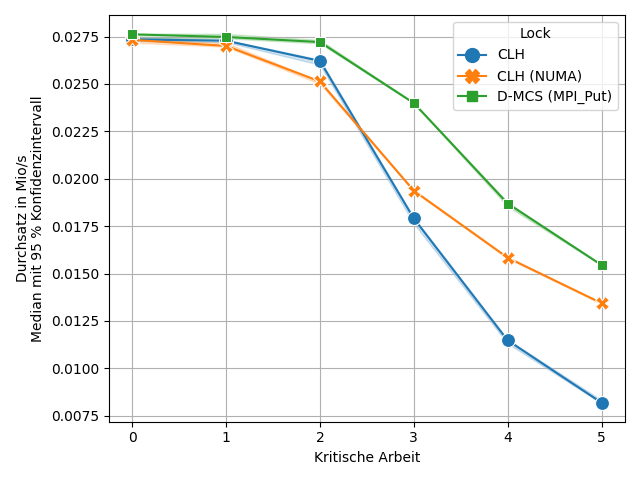
\includegraphics[width=\textwidth]{benchmarks/intelmpi/baseline/CCWB-processes=112-throughput}
        \caption{Durchsatz in Mio/s}
        \label{ben:baseline_ccwb_112_throughput}
    \end{subfigure}
    \begin{subfigure}{.5\textwidth}
        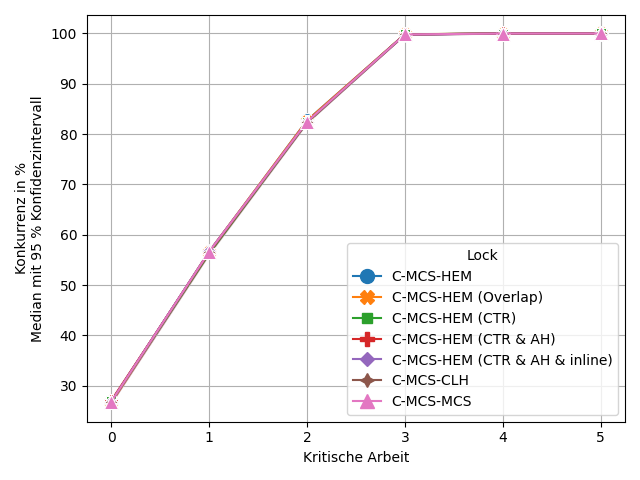
\includegraphics[width=\textwidth]{benchmarks/intelmpi/baseline/CCWB-processes=112-contention}
        \caption{Konkurrenz in \%}
        \label{ben:baseline_ccwb_112_contention}
    \end{subfigure}
    \begin{subfigure}{.5\textwidth}
        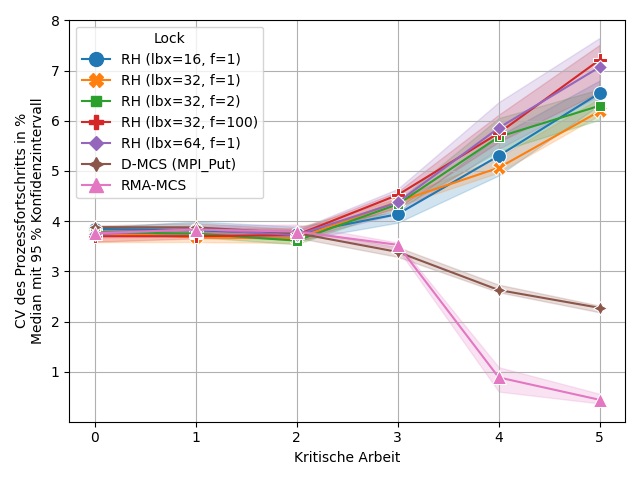
\includegraphics[width=\textwidth]{benchmarks/intelmpi/baseline/CCWB-processes=112-fairness}
        \caption{Fairness: CV des Fortschritts in \%}
        \label{ben:baseline_ccwb_112_fairness}
    \end{subfigure}
    \caption{CCWB der Basislocks mit 112 Prozessen}
    \label{ben:baseline_ccwb_112}
\end{benchmark}

\autoref{ben:baseline_ccwb_112_latency} und \autoref{ben:baseline_ccwb_112_throughput}
zeigen die Geschwindigkeit der Basislocks im \gls{ccwb} bei 112 Prozessen,
also vier voll ausgelasteten Knoten.
Ähnlich wie beim \gls{ecsb} liegen der \gls{mpi}-Lock und \texttt{dash::Mutex} nah beieinander,
während D-MCS und RMA-MCS deutlich schneller sind.
Allerdings ist in diesem Benchmark \texttt{dash::Mutex} etwas langsamer als der \gls{mpi}-Lock.
Es ist auch ersichtlich,
dass D-MCS und RMA-MCS einen deutlich geringeren Overhead haben
als die anderen beiden Locks,
da das Equilibrium bei ihnen noch nicht bei einer kritischen Arbeit von 2 einsetzt,
sondern erst später.
Dies geht auch aus \autoref{ben:baseline_ccwb_112_contention} hervor,
auch wenn die \gls{Konkurrenz} für die Locks aus den Bibliotheken \gls{mpi} und DASH nicht gemessen werden kann.

Die Fairness der Locks in \autoref{ben:baseline_ccwb_112_fairness} ist deutlich schlechter
und hat deutlich größere Konfidenzintervalle
als beim \gls{ecsb} in \autoref{ben:baseline_ecsb_fairness}.
Der Grund hierfür ist wahrscheinlich,
dass durch die geringere \gls{Konkurrenz} die Locks immer wieder frei werden.
Bei freien Locks macht es,
wie der \gls{upb} in \autoref{ben:baseline_upb} gezeigt hat,
einen großen Unterschied,
ob der akquirierende Prozess auf dem Hauptknoten läuft.
Solche Prozesse können freie Locks schneller akquirieren,
da keine entfernten Speicherzugriffe benötigt werden
und sind damit im Durchschnitt etwas schneller,
was zu einer höheren Unfairness führt.
Das erklärt auch,
warum die Fairness deutlich besser wird,
sobald das Equilibrium erreicht ist.

Darüber hinaus hat der \gls{ccwb} einen deutlich größeren Zufallsanteil,
da die Arbeit,
die jeder Prozess ausführen muss,
für jede Iteration aus einem recht großen Intervall bestimmt wird
und vollständig aus entfernten Speicherzugriffen besteht.
Auch der \gls{upb} hat bereits in \autoref{ben:baseline_upb_latency} gezeigt,
dass die Geschwindigkeit von entfernten Speicherzugriffen deutlich höheren Schwankungen unterliegt
als die von Lokalen.
Das könnte die ungenauen Konfidenzintervalle in \autoref{ben:baseline_ccwb_112_fairness} erklären.
Trotz der schlechteren Fairness haben alle Locks auch vor dem Equilibrium immer noch einen Variationskoeffizienten von unter 5~\%
und sind damit relativ fair.

\begin{benchmark}[h]
    \begin{subfigure}{.5\textwidth}
        \includegraphics[width=\textwidth]{benchmarks/intelmpi/baseline/CCWB-processes=28-latency}
        \caption{Iterationsdauer in \textmu{s}}
        \label{ben:baseline_ccwb_28_latency}
    \end{subfigure}
    \begin{subfigure}{.5\textwidth}
        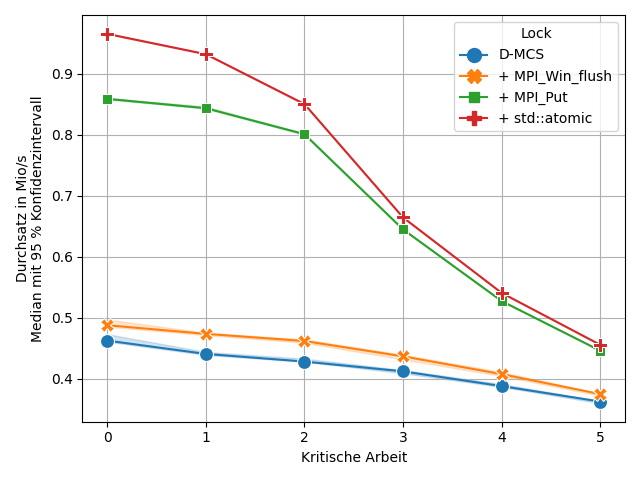
\includegraphics[width=\textwidth]{benchmarks/intelmpi/baseline/CCWB-processes=28-throughput}
        \caption{Durchsatz in Mio/s}
        \label{ben:baseline_ccwb_28_throughput}
    \end{subfigure}
    \begin{subfigure}{.5\textwidth}
        \includegraphics[width=\textwidth]{benchmarks/intelmpi/baseline/CCWB-processes=28-contention}
        \caption{Konkurrenz in \%}
        \label{ben:baseline_ccwb_28_contention}
    \end{subfigure}
    \begin{subfigure}{.5\textwidth}
        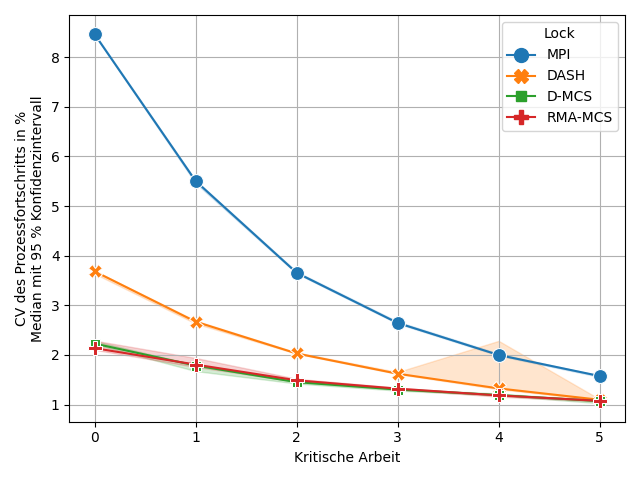
\includegraphics[width=\textwidth]{benchmarks/intelmpi/baseline/CCWB-processes=28-fairness}
        \caption{Fairness: CV des Fortschritts in \%}
        \label{ben:baseline_ccwb_28_fairness}
    \end{subfigure}
    \caption{CCWB der Basislocks mit 28 Prozessen}
    \label{ben:baseline_ccwb_28}
\end{benchmark}

Um das beim \gls{ecsb} identifizierte Optimierungspotenzial
bei der Nutzung von nur einem Knoten näher zu untersuchen,
zeigt \autoref{ben:baseline_ccwb_28} den \gls{ccwb} mit 28 Prozessen.
Da nur ein Knoten an dem Benchmark beteiligt ist,
handelt es sich bei den Operationen vor und in dem kritischen Abschnitt nun um lokale Operationen.
Da lokale Operationen deutlich schneller als entfernte Operationen sind,
sieht man den Overhead der Locks stärker.
Dabei macht es einen Unterschied,
welcher Anteil dieses Overheads auf dem kritischen Pfad (also quasi im kritischen Abschnitt)
und welcher außerhalb liegt.

Overhead außerhalb des kritischen Pfades hat denselben Effekt wie eine höhere unkritische Arbeit:
Die Iterationsdauer wird unabhängig von der Menge der kritischen Arbeit um eine Konstante erhöht.
Overhead auf dem kritischen Pfad führt zusätzlich dazu,
dass das Equilibrium früher erreicht ist,
wodurch die Iterationsdauer früher linear mit der kritischen Arbeit steigt.
Selbst wenn der Anteil der kritischen Arbeit klein ist,
ist Overhead auf dem kritischen Pfad schlechter,
weil es trotzdem passieren kann,
dass mehrere Prozesse zufällig gleichzeitig den kritischen Abschnitt betreten möchten,
wodurch sich der Overhead auf dem kritischen Pfad auf mehr als einen Prozess auswirken kann.
Umso höher der Anteil der kritischen Arbeit ist,
umso wahrscheinlicher ist es,
dass so ein Fall auftritt
und ab dem Equilibrium betrifft der Overhead auf dem kritischen Pfad immer alle Prozesse.
Umso mehr Prozesse beteiligt sind,
umso höher ist tendenziell der Anteil der kritischen Arbeit,
da sich die unkritische Arbeit auf mehr Prozesse verteilen kann (siehe auch \textit{Amdahl's Law} aus \cite{Amdahl's-law}).
Für eine gute Skalierbarkeit,
besonders im \gls{hpc}-Bereich mit Tausenden von Prozessen,
ist daher ein möglichst geringer Overhead vor allem auf dem kritischen Pfad wichtig.

\autoref{ben:baseline_ccwb_28_latency} zeigt deutlich,
dass der \gls{mpi}-Lock und \texttt{dash::Mutex} bei nur einem Knoten einen so hohen kritischen Overhead aufweisen,
dass dieser auch ohne kritische Arbeit die unkritische Arbeit von $avg(\tilde{a}) = 84$ \texttt{MPI\_Put}- und \texttt{MPI\_Get}-Operationen (jeweils mit \texttt{MPI\_Win\_flush}) dominiert.
D-MCS und RMA-MCS hingegen erreichen erst bei einer kritischen Arbeit von 1 bzw. 2 das Equilibrium,
wie \autoref{ben:baseline_ccwb_28_contention} zeigt.
Dafür weisen diese Locks einen deutlich höheren unkritischen Overhead als der \gls{mpi}-Lock auf,
sodass sie bei geringer kritischer Arbeit trotzdem langsamer sind.
Überraschenderweise ist das Equilibrium bei D-MCS und RMA-MCS nicht in \autoref{ben:baseline_ccwb_28_latency} zu sehen.
Zu erwarten wäre bei den beiden Locks ein plötzlicher starker linearer Anstieg der Iterationsdauer ab einer kritischen Arbeit von 1 bzw. 2,
mit derselben Steigung wie bei den anderen beiden Locks.
Der kritische Overhead der beiden Locks nimmt anscheinend ab,
wenn der kritische Abschnitt größer wird.
Dies wird bei der Optimierung des D-MCS in \autoref{sec:optimierung_bestehender_locks} näher untersucht.

Bei der Fairness schneidet der \gls{mpi}-Lock
mit einem Variationskoeffizienten von über 8~\%
deutlich schlechter ab
als die anderen Locks,
welche weiterhin unter 5~\% bleiben,
wie \autoref{ben:baseline_ccwb_28_fairness} zeigt.

\subsection{Vor dem Akquirieren warten (WBAB)}
\label{sec:wbab}

Der \gls{ecsb} hat gezeigt,
dass die Basislocks auf verteiltem Speicher so viel kritischen Overhead haben,
dass selbst bei leerem kritischen Abschnitt 100~\% \gls{Konkurrenz} herrscht.
Daher lässt sich die \gls{Konkurrenz} auch variieren,
indem mehr und mehr Arbeit außerhalb eines leeren kritischen Abschnitts ausgeführt wird.
Das hat gegenüber dem \gls{ccwb} den Vorteil,
dass weniger Operationen ausgeführt werden,
die zur Ungenauigkeit der Messergebnisse beitragen
und dass der Overhead des Locks einen größeren Teil der Laufzeit ausmacht,
wodurch er besser zu sehen ist.
Der Nachteil ist,
dass dieser Benchmark nicht so realistisch ist
wie der \gls{ccwb},
da ein leerer kritischer Abschnitt in der Praxis keinen Sinn macht.

Beim \gls{wbab} warten Prozesse
vor dem Akquirieren des Locks
für eine zufällig bestimmte Zeit
in einer Schleife
(\wbaburl).
Diese Zeit wird
wie beim \gls{ccwb}
aus dem geschlossenen Intervall $[w; 2w]$ bestimmt.
Dabei ist $w$
(die minimale Wartezeit in Nanosekunden)
ein Parameter des Benchmarks.
Die tatsächliche Wartezeit $\tilde{w}$ ist damit im Durchschnitt $1,5w$.
Der kritische Abschnitt ist wie beim \gls{ecsb} leer.
Anders als beim \gls{ccwb} werden in der Wartezeit vor dem kritischen Abschnitt
keine \gls{mpi}-Operationen ausgeführt.
Das ermöglicht zum einen eine beliebige Präzision,
da die Wartezeit auch in Schritten erhöht werden kann,
die kleiner sind
als eine \gls{mpi}-Operation dauert
und zum anderen eine genaue Bestimmung des Overheads bei Messung der Iterationsdauer,
da die Wartezeit in einer Zeiteinheit angegeben ist,
statt in einer Anzahl von Operationen.

Der \gls{wbab} in dieser Form kommt nicht in der Literatur über \gls{numa}-Locks vor.
Der Grund dafür ist wahrscheinlich,
dass auf gemeinsamem Speicher der Overhead der Locks geringer ist,
wodurch die \gls{Konkurrenz} bei einem leeren kritischen Abschnitt schon bei geringer Wartezeit stark abnimmt.
Bei einer Änderung der Wartezeit im Bereich von wenigen Nanosekunden
würde dann bereits die Ermittlung der Systemzeit das Messergebnis zu sehr verfälschen.
Außerdem spielt bei gemeinsamem Speicher häufig der \gls{Zwischenspeicher}-\gls{Kohaerenz}-Mechanismus eine große Rolle
und es ist wichtig zu messen,
ob der Speicher,
auf den im kritischen Abschnitt zugegriffen wird,
bereits im \gls{Zwischenspeicher} liegt.
Das ist besonders bei delegierenden Locks ein wichtiger Faktor
(siehe \autoref{sec:delegation_locks}).
In \cite{FC-MCS-Lock}, \cite{Cohort-Lock} und \cite{HMCS-Lock}
werden ähnliche Benchmarks mit einer festen Anzahl an Operationen
im kritischen Abschnitt verwendet.
Nur \cite{RMA-RW} behandelt verteilten Speicher
und nutzt einen sehr ähnlichen Benchmark mit leerem kritischen Abschnitt
und Wartezeit nach dem Freigeben des Locks.
All diese Benchmarks variieren aber die Anzahl der Prozesse und nicht die Wartezeit.
Sie nutzen eine willkürlich gewählte Wartezeit,
die unabhängig von der Anzahl der Prozesse ist.

Da bei verteiltem Speicher deutlich mehr Prozessoren zur Verfügung stehen
als bei gemeinsamem Speicher,
sollte der Benchmark auch mit beliebig vielen Prozessen ausgeführt werden können.
Daher wird beim \gls{wbab},
wie beim \gls{ccwb},
die Wartezeit abhängig von der Anzahl von Prozessen bestimmt.
Zunächst wird eine minimale Wartezeit von $w = 0$ verwendet,
um bei maximaler \gls{Konkurrenz} zu beginnen.
Dieses Szenario ist identisch zum \gls{ecsb}.
Anschließend wird $w$ so gewählt,
dass der Durchschnitt der tatsächlichen Wartezeit $\tilde{w}$,
ausgehend von $0,25~\text{\textmu{s}} \cdot p$ in jedem Schritt verdoppelt wird.
$p$ ist hierbei wieder die Anzahl der Prozesse.
Durch das exponentielle Wachstum von $\tilde{w}$ kann fast das gesamte Spektrum der \gls{Konkurrenz} untersucht werden.
Die \gls{Konkurrenz} nimmt nämlich bei zunehmender Wartezeit immer langsamer ab,
was durch das schnelle Wachstum ausgeglichen wird.

Wenn die Prozesse in der Wartezeit einfach nur in einer Schleife die Zeit prüfen,
garantiert \gls{mpi} in dieser Zeit keinen Fortschritt für andere Prozesse,
die auf den Speicher dieses Prozesses zugreifen wollen,
da ohne \gls{rdma} das Betriebssystem des Zielrechners an der Kommunikation beteiligt sein muss (vgl. \autoref{sec:mpi_fortschritt}).
Das ist vor allem ein Problem,
wenn der wartende Prozess der Hauptprozess eines Locks ist,
da die meisten Locks bei jeder Akquisition des Locks auf den Speicher dieses Prozesses zugreifen.

\begin{benchmark}[h]
    \begin{subfigure}{.5\textwidth}
        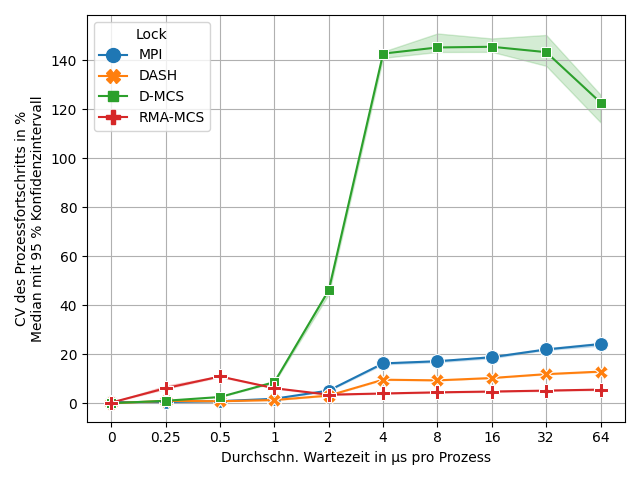
\includegraphics[width=\textwidth]{benchmarks/intelmpi/baseline/WBAB-processes=112,mpi_progress=0-fairness}
        \caption{112 Prozesse}
        \label{ben:baseline_wbab_112_no_progress_fairness}
    \end{subfigure}
    \begin{subfigure}{.5\textwidth}
        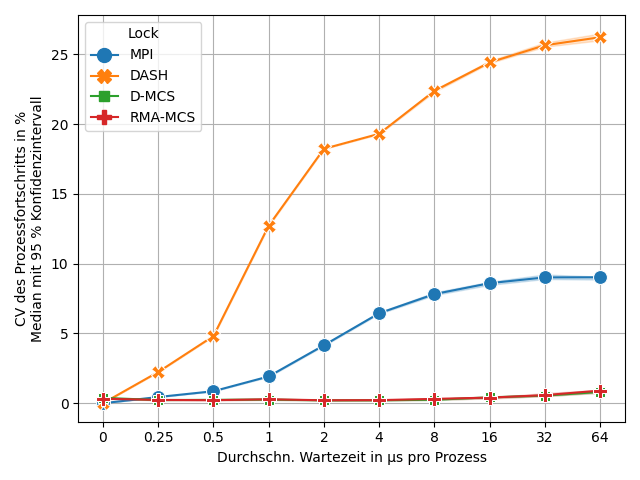
\includegraphics[width=\textwidth]{benchmarks/intelmpi/baseline/WBAB-processes=28,mpi_progress=0-fairness}
        \caption{28 Prozesse}
        \label{ben:baseline_wbab_28_no_progress_fairness}
    \end{subfigure}
    \caption{Fairness im WBAB ohne \texttt{MPI\_Iprobe}: CV des Fortschritts in \%}
    \label{ben:baseline_wbab_no_progress_fairness}
\end{benchmark}

Wie \autoref{ben:baseline_wbab_112_no_progress_fairness} zeigt,
führt das zu extremer Unfairness.
Dabei sind die Locks verschieden schwer betroffen:
D-MCS erreicht bei 112 Prozessen einen Variationskoeffizienten von mehr als 140~\%.
Das bedeutet die Standardabweichung ist über 40~\% höher als der Durchschnitt an ausgeführten Iterationen.
Die minimale Anzahl und der Median an ausgeführten Iterationen
bei einer durchschnittlichen Wartezeit von 4~\textmu{s}
waren bei D-MCS im Durchschnitt der acht Wiederholungen gerade einmal 99.25 und 102.75,
während der schnellste Prozess im Durchschnitt 1966 Iterationen schaffte.
% mean(min) 99.25
% mean(max) 1966.0
% mean(median) 102.75
Das liegt daran,
dass sich in der Wartezeit nur der Hauptprozess
(evtl. auch die anderen Prozesse auf dem Hauptknoten)
in die Warteschlange einreihen konnte.
Der Hauptprozess muss nicht nur nicht warten,
um sich in die Warteschlange einzureihen,
sondern hat im Durchschnitt auch weniger Vorgänger in der Warteschlange,
da sich in seiner Wartezeit kein anderer Prozess einreihen konnte.

\texttt{dash::Mutex} ist hiervon weniger stark betroffen,
obwohl dieser auch eine Variante des MCS-Locks ist.
Hier wird beim Freigeben des Locks immer eine \gls{cas}-Operation ausgeführt.
Auch diese kann nicht ausgeführt werden,
während der Hauptprozess wartet,
sodass in dieser Zeit gar kein Prozess kritischen Fortschritt machen kann.
Das bedeutet aber auch,
dass sich die Warteschlange in dieser Zeit nicht abbaut,
wodurch auch der Hauptprozess im Durchschnitt mehr Vorgänger hat.
Dadurch,
dass der Hauptprozess sich länger in der Warteschlange befindet,
gibt es auch ein größeres Zeitintervall,
in dem Prozesse sich in die Warteschlange einreihen können.
\texttt{dash::Mutex} wird also nicht so unfair wie D-MCS,
leidet aber auch unter massiven Einbußen bei der Geschwindigkeit.

RMA-MCS kommt von allen Locks am besten mit der Situation klar.
Da dieser Lock \gls{numa} berücksichtigt,
ist nicht bei jeder Akquisition des Locks ein Zugriff auf den Hauptprozess notwendig.
% Durch die stark reduzierte Kommunikation mit dem Hauptprozess
Dadurch hat RMA-MCS weniger Einbußen,
sowohl bei Geschwindigkeit als auch Fairness.
Nur bei einer durchschnittlichen Wartezeit von 0,5~\textmu{s} steigt der Variationskoeffizient bei RMA-MCS knapp über 10~\%.

Bei 28 Prozessen,
also auf nur einem Rechenknoten ist das Bild deutlich anders
(vgl. \autoref{ben:baseline_wbab_28_no_progress_fairness}).
Das es keine Zugriffe auf entfernten Speicher gibt,
gibt es auch keine Probleme mit Fortschrittsgarantien.
Trotzdem haben \texttt{dash::Mutex} und der Intel-MPI-Lock eine schlechte Fairness.
Der Grund hierfür ist unbekannt,
allerdings verschwindet dieser Effekt bei einer Reimplementierung des Algorithmus aus \texttt{dash::Mutex} in \autoref{sec:optimierung_bestehender_locks}.
Das erinnert an die höhere Latenz beim Akquirieren eines freien Locks
durch einen nicht-Hauptprozess auf dem Hauptknoten im \gls{upb}.
Auch dort gab es bei \texttt{dash::Mutex} und dem MPI-Lock einen Unterschied zwischen dem Hauptprozess
und anderen Prozessen auf demselben Knoten,
nicht aber bei D-MCS und RMA-MCS.
Und auch dieses Verhalten verschwindet bei einer Reimplementierung von \texttt{dash::Mutex}.

Das Szenario ist insgesamt durch den leeren kritischen Abschnitt
und der vollständigen Abwesenheit von entfernten Speicherzugriffen außerhalb des kritischen Abschnitts nicht sehr realistisch.
Trotzdem ist es in echten Anwendungen durchaus möglich,
dass Prozesse außerhalb von kritischen Abschnitten vor allem lokale Berechnungen durchführen,
die ohne \gls{mpi}-Operationen auskommen.
In solchen Fällen wäre,
genau wie in diesem Benchmark,
kein Programmfortschritt möglich.
Daher sollten bei der Verwendung von \gls{rma} in \gls{mpi}-Anwendungen lange Abschnitte ohne \gls{mpi}-Operationen vermieden werden.
Wie in \autoref{sec:mpi_fortschritt} gezeigt,
garantiert nicht jede \gls{mpi}-Operation Fortschritt.
Die Garantie hängt von der \gls{mpi}-Implementierung ab:
Weder in Intel-MPI,
noch in Open-MPI löst \texttt{MPI\_Win\_sync} das Problem,
in Open-MPI noch nicht einmal \texttt{MPI\_Win\_flush}.
Locks,
die \gls{numa} berücksichtigen,
sind hierdurch gegenüber anderen Lock-Algorithmen gleich doppelt im Vorteil.
Sie vermeiden neben langsamen entfernten Speicherzugriffen bei hinreichender \gls{Konkurrenz}
auch solche Fortschrittsprobleme.

Um die Probleme mit dem Programmfortschritt in \gls{wbab} zu lösen,
führen alle Prozesse in der Warteschleife \texttt{MPI\_Iprobe} mit \texttt{MPI\_ANY\_SOURCE} und \texttt{MPI\_ANY\_TAG} aus.
Es würde zwar reichen,
wenn nur der Hauptprozess das tun würde,
aber im Benchmark sollen alle Prozesse fair behandelt werden.
Die Ergebnisse dieser beiden Varianten unterscheiden sich tatsächlich kaum.

\begin{benchmark}[h]
    \begin{subfigure}{.5\textwidth}
        \includegraphics[width=\textwidth]{benchmarks/intelmpi/baseline/WBAB-processes=112,mpi_progress=1-latency}
        \caption{Iterationsdauer in \textmu{s}}
        \label{ben:baseline_wbab_112_latency}
    \end{subfigure}
    \begin{subfigure}{.5\textwidth}
        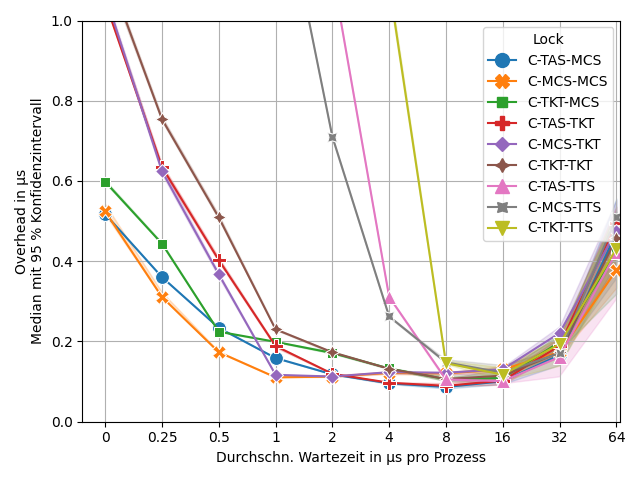
\includegraphics[width=\textwidth]{benchmarks/intelmpi/baseline/WBAB-processes=112,mpi_progress=1-overhead}
        \caption{Overhead in \textmu{s}}
        \label{ben:baseline_wbab_112_overhead}
    \end{subfigure}
    \begin{subfigure}{.5\textwidth}
        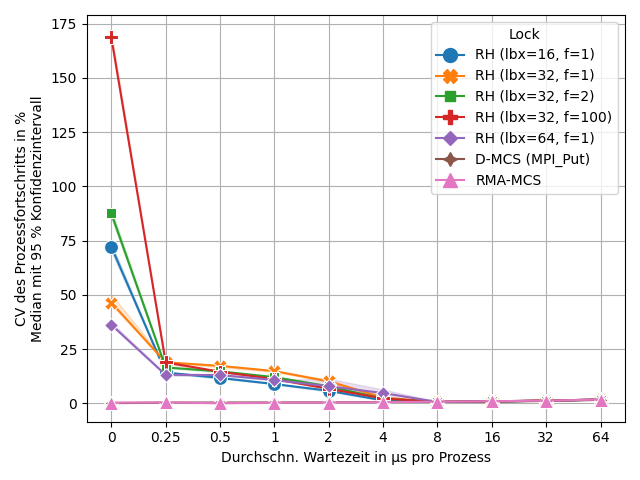
\includegraphics[width=\textwidth]{benchmarks/intelmpi/baseline/WBAB-processes=112,mpi_progress=1-fairness}
        \caption{Fairness: CV des Fortschritts in \%}
        \label{ben:baseline_wbab_112_fairness}
    \end{subfigure}
    \begin{subfigure}{.5\textwidth}
        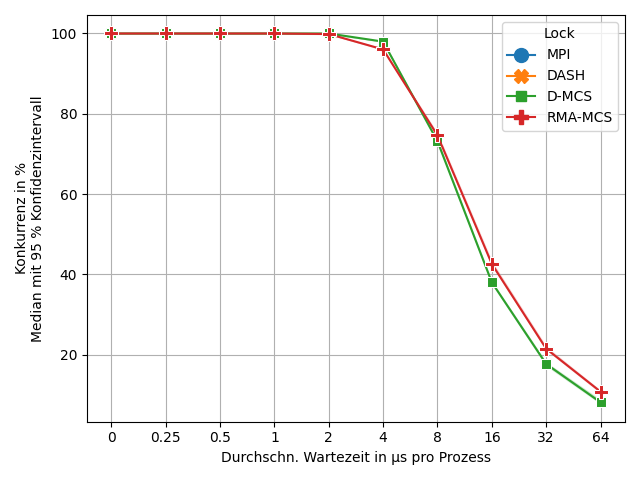
\includegraphics[width=\textwidth]{benchmarks/intelmpi/baseline/WBAB-processes=112,mpi_progress=1-contention}
        \caption{Konkurrenz in \%}
        \label{ben:baseline_wbab_112_contention}
    \end{subfigure}
    \caption{WBAB der Basislocks mit 112 Prozessen}
    \label{ben:baseline_wbab_112}
\end{benchmark}

\autoref{ben:baseline_wbab_112} zeigt die Performance der Locks im korrigierten \gls{wbab}.
Dabei sieht man in \autoref{ben:baseline_wbab_112_fairness},
dass die Fairnessprobleme durch \texttt{MPI\_Iprobe} behoben wurden:
Alle Prozesse sind fair,
mit Variationskoeffizienten von deutlich unter 2~\%.
Mit steigender Wartezeit steigt auch die Unfairness,
da Prozesse auf dem Hauptknoten etwas schneller sind.
Wenn die \gls{Konkurrenz} sinkt,
gibt es seltener eine Warteschlange,
die Fairnessgarantien durchsetzt.

Da in \autoref{ben:baseline_wbab_112_latency} sowohl die x-, als auch die y-Achse Mikrosekunden zeigen,
kann der kritische Overhead im \gls{wbab} quantifiziert werden.
Er entspricht der Iterationsdauer vor Eintreten des Equilibriums.
Das liegt daran,
dass vor Eintreten des Equilibriums die kritische Arbeit dominiert
und diese besteht im \gls{wbab} nur aus dem kritischen Overhead des Locks,
% da hier die kritische Arbeit dominiert.
% Die kritische Arbeit besteht im \gls{wbab} nur aus dem kritischen Overhead des Locks,
da der kritische Abschnitt leer ist.
% besteht die kritische Arbeit nur aus dem kritischen Overhead des Locks.
Da der kritische Overhead unabhängig von der Wartezeit ist,
bleibt auch die Iterationsdauer vor dem Einsetzen des Equilibriums relativ konstant.
Nur bei einer durchschnittlichen Wartezeit von 0~\textmu{s} gibt es größere Schwankungen.

Genau wie der \gls{ccwb},
zeigt der \gls{wbab},
dass der kritische Overhead vom \gls{mpi}-Lock und \texttt{dash::Mutex} deutlich höher ist
als der von D-MCS und RMA-MCS.
Erstere haben einen kritischen Overhead von knapp unter,
bzw. etwas über 8~\textmu{s}.
Der kritische Overhead von D-MCS und RMA-MCS ist deutlich niedriger:
bei etwa 4~\textmu{s} bzw. knapp unter 1~\textmu{s}.

\begin{benchmark}[!b]
    \begin{subfigure}{.5\textwidth}
        \includegraphics[width=\textwidth]{benchmarks/intelmpi/baseline/WBAB-processes=28,mpi_progress=1-latency}
        \caption{Iterationsdauer in \textmu{s}}
        \label{ben:baseline_wbab_28_latency}
    \end{subfigure}
    \begin{subfigure}{.5\textwidth}
        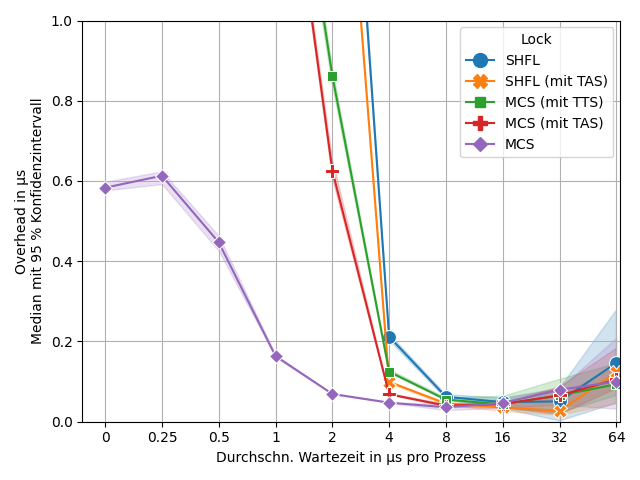
\includegraphics[width=\textwidth]{benchmarks/intelmpi/baseline/WBAB-processes=28,mpi_progress=1-overhead}
        \caption{Overhead in \textmu{s}}
        \label{ben:baseline_wbab_28_overhead}
    \end{subfigure}
    \begin{subfigure}{.5\textwidth}
        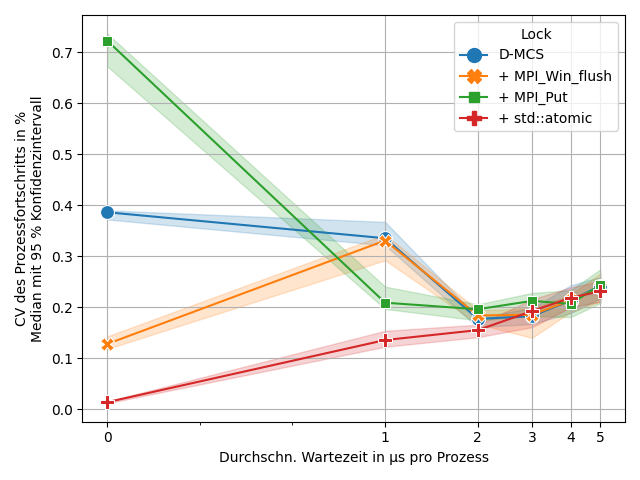
\includegraphics[width=\textwidth]{benchmarks/intelmpi/baseline/WBAB-processes=28,mpi_progress=1-fairness}
        \caption{Fairness: CV des Fortschritts in \%}
        \label{ben:baseline_wbab_28_fairness}
    \end{subfigure}
    \begin{subfigure}{.5\textwidth}
        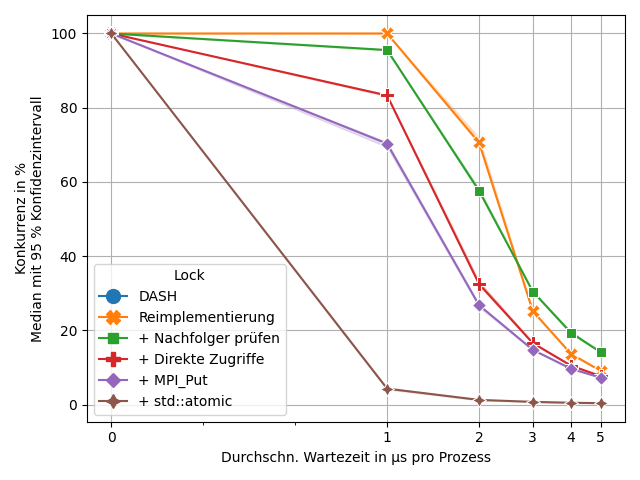
\includegraphics[width=\textwidth]{benchmarks/intelmpi/baseline/WBAB-processes=28,mpi_progress=1-contention}
        \caption{Konkurrenz in \%}
        \label{ben:baseline_wbab_28_contention}
    \end{subfigure}
    \caption{WBAB der Basislocks mit 28 Prozessen}
    \label{ben:baseline_wbab_28}
\end{benchmark}

Zusätzlich enthält \autoref{ben:baseline_wbab_112_latency} das theoretische Optimum,
welches der durchschnittlichen Wartezeit entspricht.
Da bei \gls{wbab} das theoretische Optimum bekannt ist,
kann der reine Overhead der Locks gezeigt werden,
indem das Optimum von der Iterationsdauer abgezogen wird.
Dieser Overhead wird in \autoref{ben:baseline_wbab_112_overhead} gezeigt.
Im Gegensatz zu \autoref{ben:baseline_wbab_112_latency},
geht hier die durchschnittliche Wartezeit bis 64~\textmu{s} pro Prozess,
wodurch die \gls{Konkurrenz} auf etwa 10~\% fällt
(vgl. \autoref{ben:baseline_wbab_112_contention}).
Eine noch höhere Wartezeit würde zwar die \gls{Konkurrenz} noch weiter senken,
aber eine Wartezeit von $64~\text{\textmu{s}} \cdot 112 \approx 7~\text{ms}$ ist bereits so groß,
dass das Messergebnis ungenau wird,
wie die Konfidenzintervalle zeigen.
Bei einer Laufzeit von einer Sekunde,
wobei 10~\% auch noch zum Aufwärmen verwendet werden,
schafft jeder Prozess bei dieser Wartezeit nur noch etwa 125 Iterationen.
Hinzu kommt,
dass bei sehr geringer \gls{Konkurrenz} immer mehr Zugriffe auf entfernten Speicher zum Overhead beitragen.
Das liegt daran,
dass immer mehr freie Locks akquiriert werden müssen
und die meisten Prozesse auf einem anderen Knoten laufen
als der Hauptprozess.
Entfernte Zugriffe haben größere Schwankungen,
was die Ungenauigkeit weiter erhöht.
Da sie auch langsam sind,
nimmt der Overhead ab einer \gls{Konkurrenz} von 40~\% wieder zu.

Die Betrachtung des Overheads auch bei höheren Wartezeiten zeigt,
dass auch nach Erreichen des Equilibriums der Overhead zunächst weiter abnimmt
und später wieder steigt.
Dabei sieht man in \autoref{ben:baseline_wbab_112_overhead},
dass bei geringer \gls{Konkurrenz} der D-MCS-Lock etwas besser ist
als der RMA-MCS-Lock.
Genau wie beim \gls{upb} sieht man hier den Nachteil der zwei Hierarchieebenen des RMA-MCS-Locks,
durch die ein Prozess bei geringer \gls{Konkurrenz} oft beide MCS-Locks nacheinander akquirieren muss,
was natürlich langsamer ist
als nur einen MCS-Lock zu akquirieren,
so wie es bei D-MCS der Fall ist.
Da einer der Locks aber nur lokal ist,
ist dieser Nachteil sehr klein.

Der Vollständigkeit halber zeigt \autoref{ben:baseline_wbab_28} den \gls{wbab} mit 28 Prozessen.
Wie auch in \gls{ecsb} und \gls{ccwb} ist der MPI-Lock bei nur einem Rechenknoten deutlich am schnellsten.
D-MCS und RMA-MCS sind nah beieinander auf Platz zwei und drei
und \texttt{dash::Mutex} am langsamsten.
Die Fairness ist wie bei 112 Prozessen mit einem Variationskoeffizienten von deutlich unter 1~\% sehr gut.

\section{Optimierung bestehender Locks}
\label{sec:optimierung_bestehender_locks}

Bevor \gls{numa}-Algorithmen auf verteilten Speicher portiert werden,
werden die in \autoref{ch:dist_locks} identifizierten Optimierungen auf die bestehenden Locks angewandt.
So können diese bei der Portierung direkt berücksichtigt werden.

Die bestehenden Locks enthalten zwei Varianten,
einen Lock weiterzugeben:
D-MCS und RMA-MCS nutzen hierfür \gls{rma},
während \texttt{dash::Mutex} hierfür Punkt-zu-Punkt-Kommunika-tion nutzt.
Um beide Varianten fair evaluieren zu können,
werden D-MCS in \autoref{sec:optimierung_dmcs} und \texttt{dash::Mutex} in \autoref{sec:optimierung_dash} optimiert.

In diesem Abschnitt wird der \gls{wbab} mit linear statt exponentiell steigender Wartezeit ausgeführt,
da für die Vergleiche vor allem die Iterationsdauer interessant ist
und so eine höhere Auflösung bei geringen Werten vorliegt.

\subsection{Optimierung von D-MCS}
\label{sec:optimierung_dmcs}

Der D-MCS-Lock ist bereits ein sehr optimierter Lock.
Dennoch wurden in dieser Arbeit einige Verbesserungen identifiziert,
die bereits in \autoref{fig:mcs_mpi_code} gezeigt wurden.

Erstens nutzt D-MCS nach Aufrufen von \texttt{MPI\_Accumulate} kein \texttt{MPI\_Win\_flush}
und auch keine sonstige Synchronisierungsfunktion.
Das betrifft zum einen das Benachrichtigen des Vorgängers beim Einreihen in die Warteschlange
und zum anderen die letzte Operation beim Weitergeben des Locks an einen Nachfolger.
Ohne Synchronisierungsfunktion ist aber nicht garantiert,
dass diese Operation überhaupt ausgeführt wird:

\clearpage

\foreignblockcquote{english}[Kapitel 11.7.3, S. 462]{MPI-3.1}{%
    \textins{A}n RMA communication may become enabled as soon as the corresponding
    put, get or accumulate call has executed, or as late as when the ensuing synchronization
    call is issued.}
Außerdem verletzt das \texttt{MPI\_Accumulate},
welches den Lock an den Nachfolger übergibt,
die \gls{mpi}-Spezifikation:
\foreignblockcquote{english}[Kapitel 11.3, S. 417]{MPI-3.1}{%
    \textins{RMA} operations are nonblocking: the
    call initiates the transfer, but the transfer may continue after the call returns. The transfer
    is completed, at the origin or both the origin and the target, when a subsequent synchronization
    call is issued by the caller on the involved window object \textelp{}.
    The local communication buffer of an RMA call should not be updated \textelp{} after the RMA call until the
    operation completes at the origin.}
Da es die letzte Operation in der \texttt{release}-Funktion ist,
wird nach dieser Operation der Speicher auf dem Stack freigegeben,
der an \texttt{MPI\_Accumulate} übergeben wurde.
Je nachdem,
wann die \gls{mpi}-Implementierung auf diesen Speicher zugreift,
ist der Speicher also invalide.

\begin{benchmark}[h]
    \begin{subfigure}{.5\textwidth}
        \includegraphics[width=\textwidth]{benchmarks/intelmpi/dmcs-optimization/UPB-lock_count=1000-latency}
        \caption{UPB}
        \label{ben:dmcs_upb_latency}
    \end{subfigure}
    \begin{subfigure}{.5\textwidth}
        \includegraphics[width=\textwidth]{benchmarks/intelmpi/dmcs-optimization/ECSB-latency}
        \caption{ECSB}
        \label{ben:dmcs_ecsb_latency}
    \end{subfigure}
    \begin{subfigure}{.5\textwidth}
        \includegraphics[width=\textwidth]{benchmarks/intelmpi/dmcs-optimization/CCWB-processes=112-latency}
        \caption{CCWB mit 112 Prozessen}
        \label{ben:dmcs_ccwb_112_latency}
    \end{subfigure}
    \begin{subfigure}{.5\textwidth}
        \includegraphics[width=\textwidth]{benchmarks/intelmpi/dmcs-optimization/WBAB-processes=112,mpi_progress=1-latency}
        \caption{WBAB mit 112 Prozessen}
        \label{ben:dmcs_wbab_112_latency}
    \end{subfigure}
    \caption{Iterationsdauer der D-MCS-Optimierungen in \textmu{s}}
    \label{fig:dmcs_latency}
\end{benchmark}

Als Korrektur und erste Optimierung werden daher beide \texttt{MPI\_Accumulate}-Operationen direkt im Anschluss mit \texttt{MPI\_Win\_flush} vollständig ausgeführt.
Zwar würde eine lokale Ausführung mit \texttt{MPI\_Win\_flush\_local} reichen,
aber da sich die Operationen jeweils auf dem kritischen Pfad befinden,
ist eine direkte vollständige Ausführung wünschenswert.

\autoref{fig:dmcs_latency} zeigt,
dass diese Änderung einen interessanten Effekt hat:
Wenn keine Arbeit ausgeführt wird,
wie es im \gls{ecsb} (vgl. \autoref{ben:dmcs_ecsb_latency})
und \gls{wbab} (vgl. \autoref{ben:dmcs_wbab_112_latency}) ohne Wartezeit der Fall ist,
wird der Lock langsamer.
Ansonsten wird er schneller.
Dies ist in \autoref{ben:dmcs_ccwb_112_latency} allerdings kaum zu erkennen,
da die Verbesserung nur klein ist.

Die Verbesserung ist von der unkritischen Arbeit abhängig,
da ohne unkritische Arbeit der Lock direkt wieder akquiriert wird,
wobei auch \texttt{MPI\_Win\_flush} zum Einsatz kommt.
In diesem Fall verursacht die Änderung also nur unnötigen Overhead.
Wenn aber zunächst unkritische Arbeit ausgeführt wird,
kann sich dadurch die Ausführung von \texttt{MPI\_Accumulate} verzögern
und damit der kritische Pfad verlängern.

Die zweite Optimierung ist die nicht-atomare Übergabe von Locks aus \autoref{sec:non_atomic_lock_passing}.
Statt der beiden \texttt{MPI\_Accumulate}-Operationen wird \texttt{MPI\_Put} verwendet.
Dadurch muss die \gls{mpi}-Implementierung nicht mehr prüfen,
ob mehrere parallele \gls{rma}-Operationen auf diesen Speicherbereich zugreifen.
Parallele Zugriffe sind an diesen Stellen sowieso durch den Algorithmus ausgeschlossen.
% Das kann auch tatsächlich in beiden Fällen nicht der Fall sein.
Die Optimierung realisiert auch das in \autoref{sec:ecsb} identifizierte Optimierungspotenzial auf einem einzelnen Rechenknoten.
Sowohl in \autoref{ben:dmcs_ecsb_latency}
als auch in \autoref{ben:dmcs_ccwb_28} wird das deutlich.
Der so optimierte D-MCS schlägt sogar den Intel-MPI-Lock,
welcher auf einem Rechenknoten zuvor die beste Performance hatte
(siehe \autoref{ben:baseline_opt_ccwb_28_latency}).

\begin{benchmark}[h]
    \begin{subfigure}{.5\textwidth}
        \includegraphics[width=\textwidth]{benchmarks/intelmpi/dmcs-optimization/CCWB-processes=28-latency}
        \caption{Iterationsdauer in \textmu{s}}
        \label{ben:dmcs_ccwb_28_latency}
    \end{subfigure}
    \begin{subfigure}{.5\textwidth}
        \includegraphics[width=\textwidth]{benchmarks/intelmpi/dmcs-optimization/CCWB-processes=28-contention}
        \caption{Konkurrenz in \%}
        \label{ben:dmcs_ccwb_28_contention}
    \end{subfigure}
    \caption{CCWB der D-MCS-Optimierungen mit 28 Prozessen}
    \label{ben:dmcs_ccwb_28}
\end{benchmark}

Die letzte Optimierung ist das Ersetzen der \gls{mpi}-Operationen durch C++ \texttt{std::atomic}.
Damit ist zwar nur lokale,
also auf den Knoten beschränkte Kommunikation möglich,
aber wie in \autoref{sec:mpi_shared_mem} erwähnt,
kann so ein Lock als Baustein für \gls{numa}-Locks wie den Cohort-Lock \cite{Cohort-Lock} dienen.
Außerdem wird hierdurch noch einmal verdeutlicht,
welchen Overhead die lokale Nutzung von \gls{rma}-Operationen mit sich bringt.
Das ist besonders in \autoref{ben:dmcs_upb_latency} ersichtlich.

\clearpage

\subsection{Optimierung von dash::Mutex}
\label{sec:optimierung_dash}

Damit der Algorithmus von \texttt{dash::Mutex} leichter optimiert werden kann,
wird er zunächst wie die anderen Locks mit einem eigenen \gls{mpi}-\gls{Fenster} reimplementiert.
Der Quelltext der Reimplementierung ist in \autoref{fig:dash_code} zu sehen.
Dabei ändern sich einige Implementierungsdetails
und da der Lock nun nicht mehr in die Bibliothek DASH eingebunden ist,
entfallen einige lokale Operationen,
wie etwa das Laden von Metadaten des DASH-Teams.

\begin{figure}[h]
    \begin{subfigure}{.5\textwidth}
        \centering
        \begin{tabular}{c}\begin{lstlisting}
win_mem->next = -1;
MPI_Win_sync(win);

// Finde Vorgänger
int pred;
MPI_Fetch_and_op(
  &my_rank, &pred, MPI_INT,
  main_rank, tail_disp,
  MPI_REPLACE, win);
MPI_Win_flush(main_rank, win);

if (pred != -1) {
  // Reihe nach Vorgänger ein
  int result;
  MPI_Fetch_and_op(
    &my_rank, &result, MPI_INT,
    pred, next_disp,
    MPI_REPLACE, win);
  MPI_Win_flush(pred, win);

  // Warte auf Vorgänger
  MPI_Recv(NULL, 0, MPI_UINT8_T,
           predecessor, 0, comm,
           MPI_STATUS_IGNORE);
}
        \end{lstlisting}\end{tabular}
        \caption{Akquirieren des Locks (\texttt{acquire})}
        \label{fig:dash_acquire}
    \end{subfigure}
    \begin{subfigure}{.5\textwidth}
        \centering
        \begin{tabular}{c}\begin{lstlisting}
constexpr int NULL_RANK = -1;
int old_value;
MPI_Compare_and_swap(
  &NULL_RANK, &my_rank, &old_value,
  MPI_INT, main_rank, tail_disp, win);
MPI_Win_flush(main_rank, win);

// Die Warteschlange ist leer
if (old_value == my_rank) return;
// Warte auf Nachfolger
int succ;
do {
  int flag; // Garantiere Fortschritt
  MPI_Iprobe(
    MPI_ANY_SOURCE, MPI_ANY_TAG,
    comm, &flag, MPI_STATUS_IGNORE);

  MPI_Fetch_and_op(
    NULL, &successor, MPI_INT,
    my_rank, next_disp, MPI_NO_OP, win);
  MPI_Win_flush(my_rank, win);
} while(succ == -1);
// Benachrichtige Nachfolger
MPI_Send(NULL, 0, MPI_UINT8_T,
         successor, 0, comm);
        \end{lstlisting}\end{tabular}
        \caption{Freigeben des Locks (\texttt{release})}
        \label{fig:dash_release}
    \end{subfigure}
    \caption{Implementierung von \texttt{dash::Mutex}}
    \label{fig:dash_code}
\end{figure}

Durch das Entfallen dieser Operationen nimmt vor allem der unkritische Overhead ab.
Das sieht man besonders im \gls{ccwb} und \gls{wbab} auf einem Rechenknoten
(in \autoref{ben:dash_ccwb_28_latency} und \autoref{ben:dash_wbab_28_latency}):
Beide Implementierungen erreichen bei einer kritischen Arbeit von 0,
bzw. einer Wartezeit von 2~\textmu{s} das Equilibrium,
haben also vergleichbaren kritischen Overhead,
die Reimplementierung ist aber immer etwas schneller.
Durch diese Reimplementierung verschwindet auch das in \autoref{sec:upb} festgestellte Verhalten,
dass das Akquirieren eines freien Locks länger dauert,
wenn es sich nicht um den Hauptprozess handelt (siehe \autoref{ben:dash_upb_latency}).

\begin{benchmark}[!h]
    \begin{subfigure}{.5\textwidth}
        \includegraphics[width=\textwidth]{benchmarks/intelmpi/dash-optimization/UPB-lock_count=1000-latency}
        \caption{UPB}
        \label{ben:dash_upb_latency}
    \end{subfigure}
    \begin{subfigure}{.5\textwidth}
        \includegraphics[width=\textwidth]{benchmarks/intelmpi/dash-optimization/ECSB-latency}
        \caption{ECSB}
        \label{ben:dash_ecsb_latency}
    \end{subfigure}
    \begin{subfigure}{.5\textwidth}
        \includegraphics[width=\textwidth]{benchmarks/intelmpi/dash-optimization/CCWB-processes=28-latency}
        \caption{CCWB mit 28 Prozessen}
        \label{ben:dash_ccwb_28_latency}
    \end{subfigure}
    \begin{subfigure}{.5\textwidth}
        \includegraphics[width=\textwidth]{benchmarks/intelmpi/dash-optimization/WBAB-processes=28,mpi_progress=1-latency}
        \caption{WBAB mit 28 Prozessen}
        \label{ben:dash_wbab_28_latency}
    \end{subfigure}
    \begin{subfigure}{.5\textwidth}
        \includegraphics[width=\textwidth]{benchmarks/intelmpi/dash-optimization/CCWB-processes=112-latency}
        \caption{CCWB mit 112 Prozessen}
        \label{ben:dash_ccwb_112_latency}
    \end{subfigure}
    \begin{subfigure}{.5\textwidth}
        \includegraphics[width=\textwidth]{benchmarks/intelmpi/dash-optimization/WBAB-processes=112,mpi_progress=1-latency}
        \caption{WBAB mit 112 Prozessen}
        \label{ben:dash_wbab_112_latency}
    \end{subfigure}
    \caption{Iterationsdauer der DASH-Optimierungen in \textmu{s}}
    \label{fig:dash_latency}
\end{benchmark}

Das Hauptproblem an dem Algorithmus hinter \texttt{dash::Mutex} ist,
dass in \texttt{release} nicht,
wie bei einem MCS-Lock üblich,
mit einer lokalen Operation geprüft wird,
ob sich bereits ein Nachfolger registriert hat.
Stattdessen wird direkt versucht,
mit einer \gls{cas}-Operation auf den entfernten Speicher des Hauptprozesses
den Lock freizugeben.
Erst wenn diese Operation fehlschlägt,
wird mit \texttt{MPI\_Fetch\_and\_op} und \texttt{MPI\_NO\_OP} auf einen lokalen Nachfolger gewartet (\autoref{fig:dash_release}, Zeile 10-22).
Die erste Optimierung besteht daher darin,
in \texttt{release} bereits vor dem \gls{cas} mit \texttt{MPI\_Fetch\_and\_op} und \texttt{MPI\_NO\_OP} atomar zu prüfen,
ob lokal ein Nachfolger registriert ist.
Hier wird eine atomare \gls{mpi}-Funktion benötigt,
um einen \textit{memory consistency error} zu vermeiden,
wenn der Nachfolger genau im selben Moment Zeile 13-19 in \autoref{fig:dash_acquire} ausführt,
um sich zu registrieren.

Der \gls{upb} zeigt in \autoref{ben:dash_upb_latency},
dass diese Änderung bei einem freien Lock etwas langsamer ist,
da eine zusätzliche Operation ausgeführt wird,
die unnötig ist,
wenn es keinen Nachfolger gibt.
Da es sich aber nur um eine Lese-Operation handelt,
ist dieser zusätzliche Overhead sehr gering,
besonders wenn man ihn mit dem Overhead der Einbettung in DASH vergleicht.
Dafür verbessert diese Änderung die Performance in allen anderen Benchmarks drastisch:
Wenn es einen Nachfolger gibt,
wird eine \gls{cas}-Operation vermieden,
die deutlich langsamer ist als die atomare Lese-Operation,
die in diesem Fall sowieso im Anschluss ausgeführt würde.
Wenn mehrere Knoten beteiligt sind,
ist dieser Effekt sogar noch stärker,
da die \gls{cas}-Operation auf den Speicher des Hauptprozesses
und damit potenziell auf entfernten Speicher zugreift.

Als zweite Optimierung werden,
wie im D-MCS-Lock,
für Zugriffe auf lokalen Speicher direkte Speicherzugriffe verwendet (vgl. \autoref{fig:mcs_mpi_release}, Zeile 13-20).
Das betrifft nur das in der ersten Optimierung hinzugefügte \texttt{MPI\_Fetch\_and\_op}
und das Warten auf den Nachfolger (\autoref{fig:dash_release}, Zeile 18-21),
da \texttt{dash::Mutex} Punkt-zu-Punkt-Kommunikation für die Lockübergabe nutzt.
Diese Optimierung gleicht die kleine Verschlechterung im \gls{upb} wieder aus,
da ein direkter lesender Zugriff auf lokalen Speicher sehr schnell ist,
und auch in allen anderen Benchmarks verbessert sich dadurch die Geschwindigkeit.

Als drittes wird wie in \autoref{sec:optimierung_dmcs} \texttt{MPI\_Put} verwendet,
um sich beim Vorgänger zu registrieren (\autoref{fig:dash_acquire}, Zeile 15-18).
Anders als bei D-MCS ersetzt \texttt{MPI\_Put} hier ein \texttt{MPI\_Fetch\_and\_op} und nicht ein \texttt{MPI\_Accumulate}.
Warum \texttt{dash::Mutex} an dieser Stelle \texttt{MPI\_Fetch\_and\_op} verwendet ist nicht klar.
Diese Funktion liefert im Gegensatz zu \texttt{MPI\_Accumulate} den Wert zurück,
der vor der Operation an der Speicheradresse stand.
Dieser alte Wert (die lokale Variable \texttt{result}) wird aber gar nicht verwendet.
Diese Optimierung bringt anders als bei D-MCS nur eine relativ kleine Verbesserung bei mehreren Rechenknoten,
da die Übergabe des Locks an den Nachfolger Punkt-zu-Punkt-Kommunikation nutzt
und somit nicht betroffen ist.
Nach dem Registrieren beim Vorgänger müssen Prozesse typischerweise sowieso auf ihren Vorgänger warten.
Daher bringt es nichts,
wenn das Registrieren schneller ist.
Trotzdem verbessert sich die Performance bei nur einem Rechenknoten deutlich.
Zu prüfen,
ob mehrere parallele \gls{rma}-Operationen auf denselben Speicherbereich zugreifen,
verursacht demnach erheblichen Overhead bei der \gls{mpi}-Implementierung.

Als letzte Optimierung werden wieder alle \gls{mpi}-Operationen durch C++ \texttt{std::atomic} ersetzt,
wodurch dieser Lock wieder nur als Baustein für \gls{numa}-Locks wie den Cohort-Lock \cite{Cohort-Lock} dienen kann.

\begin{benchmark}[h]
    \begin{subfigure}{.5\textwidth}
        \includegraphics[width=\textwidth]{benchmarks/intelmpi/baseline-opt/CCWB-processes=28-latency}
        \caption{28 Prozesse}
        \label{ben:baseline_opt_ccwb_28_latency}
    \end{subfigure}
    \begin{subfigure}{.5\textwidth}
        \includegraphics[width=\textwidth]{benchmarks/intelmpi/baseline-opt/CCWB-processes=112-latency}
        \caption{112 Prozesse}
        \label{ben:baseline_opt_ccwb_112_latency}
    \end{subfigure}
    \caption{CCWB der Basislocks-Optimierungen: Iterationsdauer in \textmu{s}}
    \label{ben:baseline_opt_ccwb}
\end{benchmark}

\clearpage

\autoref{ben:baseline_opt_ccwb} zeigt schließlich die optimierten Varianten von D-MCS und \texttt{dash::Mutex} noch einmal im Vergleich miteinander
und zusätzlich im Vergleich zu dem Intel-MPI-Lock und RMA-MCS auf einem und vier Rechenknoten.
In \autoref{ben:baseline_opt_ccwb_28_latency} sieht man,
dass bei einem Knoten der optimierte D-MCS,
also \gls{rma},
schneller ist.
\autoref{ben:baseline_opt_ccwb_112_latency} zeigt,
dass bei mehreren Knoten hingegen der optimierte \texttt{dash::Mutex},
also Punkt-zu-Punkt-Kommunikation,
schneller ist.
Beide optimierte Varianten schlagen den Intel-MPI-Lock,
welcher zuvor auf einem Rechenknoten am schnellsten war,
aber trotz aller Optimierungen erreicht bei mehreren Rechenknoten weiterhin keiner der Locks die Geschwindigkeit von RMA-MCS.
Das zeigt deutlich das enorme Potenzial der Portierung von \gls{numa}-Locks auf verteilten Speicher.
